% ============================================================
%  03_thietke.tex – Chương 3: Thiết kế hệ thống
% ============================================================
\chapter{Thiết Kế Hệ Thống}

\section{Chuyển Từ Phân Tích Sang Thiết Kế}

Từ các use case ở Chương 2, hệ thống được chia thành ba nhóm trách nhiệm: giao tiếp người dùng, điều phối nghiệp vụ và hạ tầng dữ liệu. Các danh từ miền nghiệp vụ như sản phẩm, biến thể, nguyên liệu, đơn hàng và quyền được chuyển thành lớp hoặc module; các động từ như tìm kiếm, đặt hàng, kiểm tra tồn và duyệt nội dung được chuyển thành API, workflow hoặc subscriber. Biểu đồ lớp miền mô tả cấu trúc ổn định, biểu đồ hoạt động mô tả trách nhiệm giữa các vùng xử lý, còn biểu đồ trình tự làm rõ thứ tự gọi tại runtime.

\section{Kiến Trúc Tổng Thể}

Hệ thống áp dụng kiến trúc headless commerce. Giao diện React không truy cập cơ sở dữ liệu trực tiếp mà giao tiếp với Medusa qua JS SDK và các API tùy biến. Các dịch vụ dữ liệu được triển khai độc lập, nhờ đó có thể thay đổi giao diện hoặc mở rộng hạ tầng mà không làm thay đổi toàn bộ lõi nghiệp vụ.

\begin{figure}[H]
  \centering
  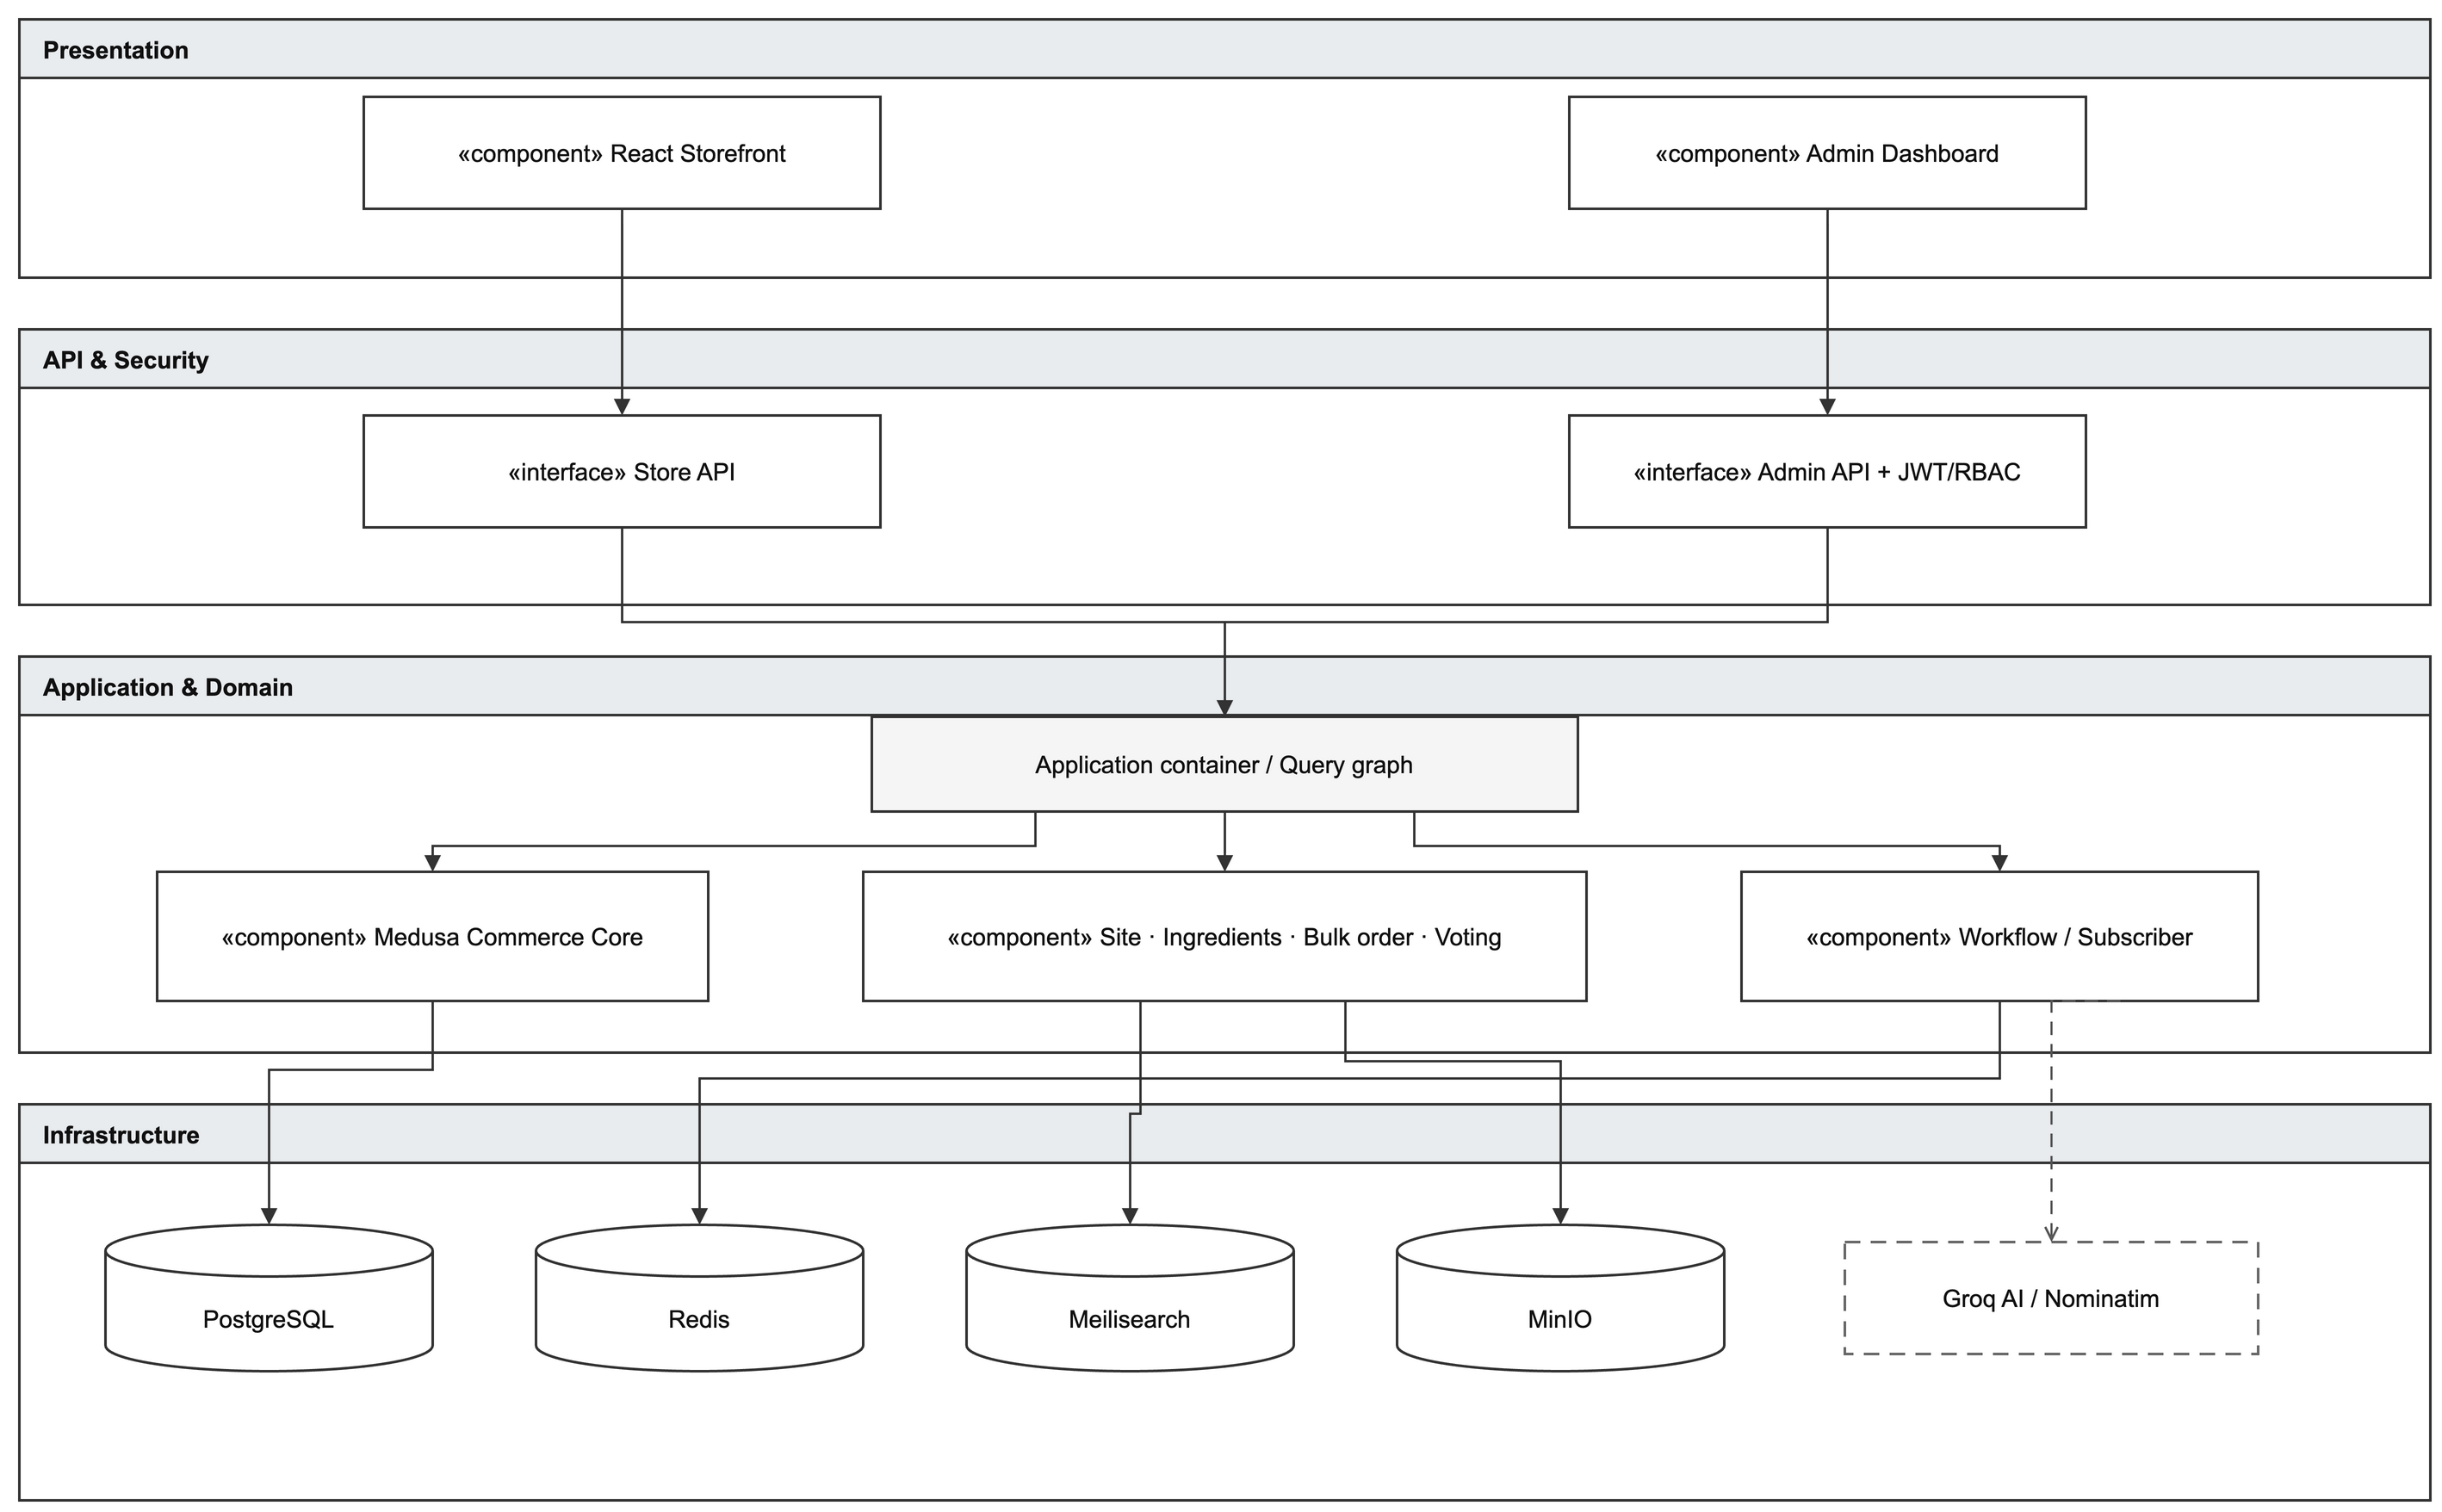
\includegraphics[width=\textwidth,height=0.74\textheight,keepaspectratio]{images/architecture.drawio.png}
  \caption{Kiến trúc logic của Mọng Fruitboxz}
  \label{fig:architecture}
\end{figure}

\section{Thiết Kế Frontend}

\subsection{Tổ chức ứng dụng}

Frontend được xây dựng dưới dạng single-page application. \techterm{React Router} ánh xạ URL tới trang; \techterm{React.lazy} và \techterm{Suspense} tách bundle theo route. Các provider ở cấp ứng dụng quản lý catalog, giỏ hàng, ngôn ngữ, xác thực khách hàng và xác thực quản trị.

\begin{longtable}{@{}p{0.25\textwidth} p{0.67\textwidth}@{}}
  \toprule
  \textbf{Thành phần} & \textbf{Trách nhiệm} \\
  \midrule
  \endhead
  \texttt{apiFetch} & Bọc \texttt{medusa.client.fetch}, tự xử lý timeout, token và cấu trúc response envelope. \\
  \texttt{CatalogContext} & Cung cấp dữ liệu sản phẩm và danh mục cho các trang mua sắm. \\
  \texttt{CartContext} & Quản lý reducer giỏ hàng, localStorage, đồng bộ Redis và thông báo thêm hàng. \\
  \texttt{AuthContext} & Đọc JWT khách hàng, kiểm tra hết hạn và cung cấp trạng thái đăng nhập. \\
  \texttt{AdminAuthContext} & Đăng nhập admin, tải quyền, xử lý 401 và kiểm tra quyền theo chức năng. \\
  \texttt{LanguageContext} & Kết hợp i18next để hỗ trợ nội dung tiếng Việt và tiếng Anh. \\
  \bottomrule
\end{longtable}

\subsection{Nguyên tắc giao tiếp API}

Medusa SDK được cấu hình với backend URL, publishable key và cơ chế lưu JWT. API lõi và API tùy biến đều đi qua một lớp gọi chung để nhất quán timeout và xử lý lỗi. Riêng tìm kiếm có thể gọi Meilisearch trực tiếp khi cấu hình search key phía client; nếu không, giao diện gọi API backend.

\section{Thiết Kế Backend Medusa}

\subsection{Mô-đun lõi và mô-đun mở rộng}

Medusa cung cấp các mô-đun lõi như Product, Pricing, Inventory, Order, Customer, User, Promotion và Region. Dự án đăng ký thêm năm mô-đun:

\begin{itemize}[leftmargin=2em, itemsep=4pt]
  \item \textbf{Site:} banner, cấu hình website, blog, liên hệ và log chatbot.
  \item \textbf{RBAC:} role, permission và ánh xạ quyền của người dùng quản trị.
  \item \textbf{Ingredients:} nguyên liệu, công thức BOM và kiểm tra/trừ tồn kho.
  \item \textbf{Bulk orders:} lưu yêu cầu đặt hàng số lượng lớn.
  \item \textbf{Voting:} điểm và bình luận gắn với khách hàng, sản phẩm.
\end{itemize}

Các module link nối User với Role và Ingredient với InventoryItem mà không đưa khóa ngoại của mô-đun khác trực tiếp vào model tùy biến.

\begin{figure}[H]
  \centering
  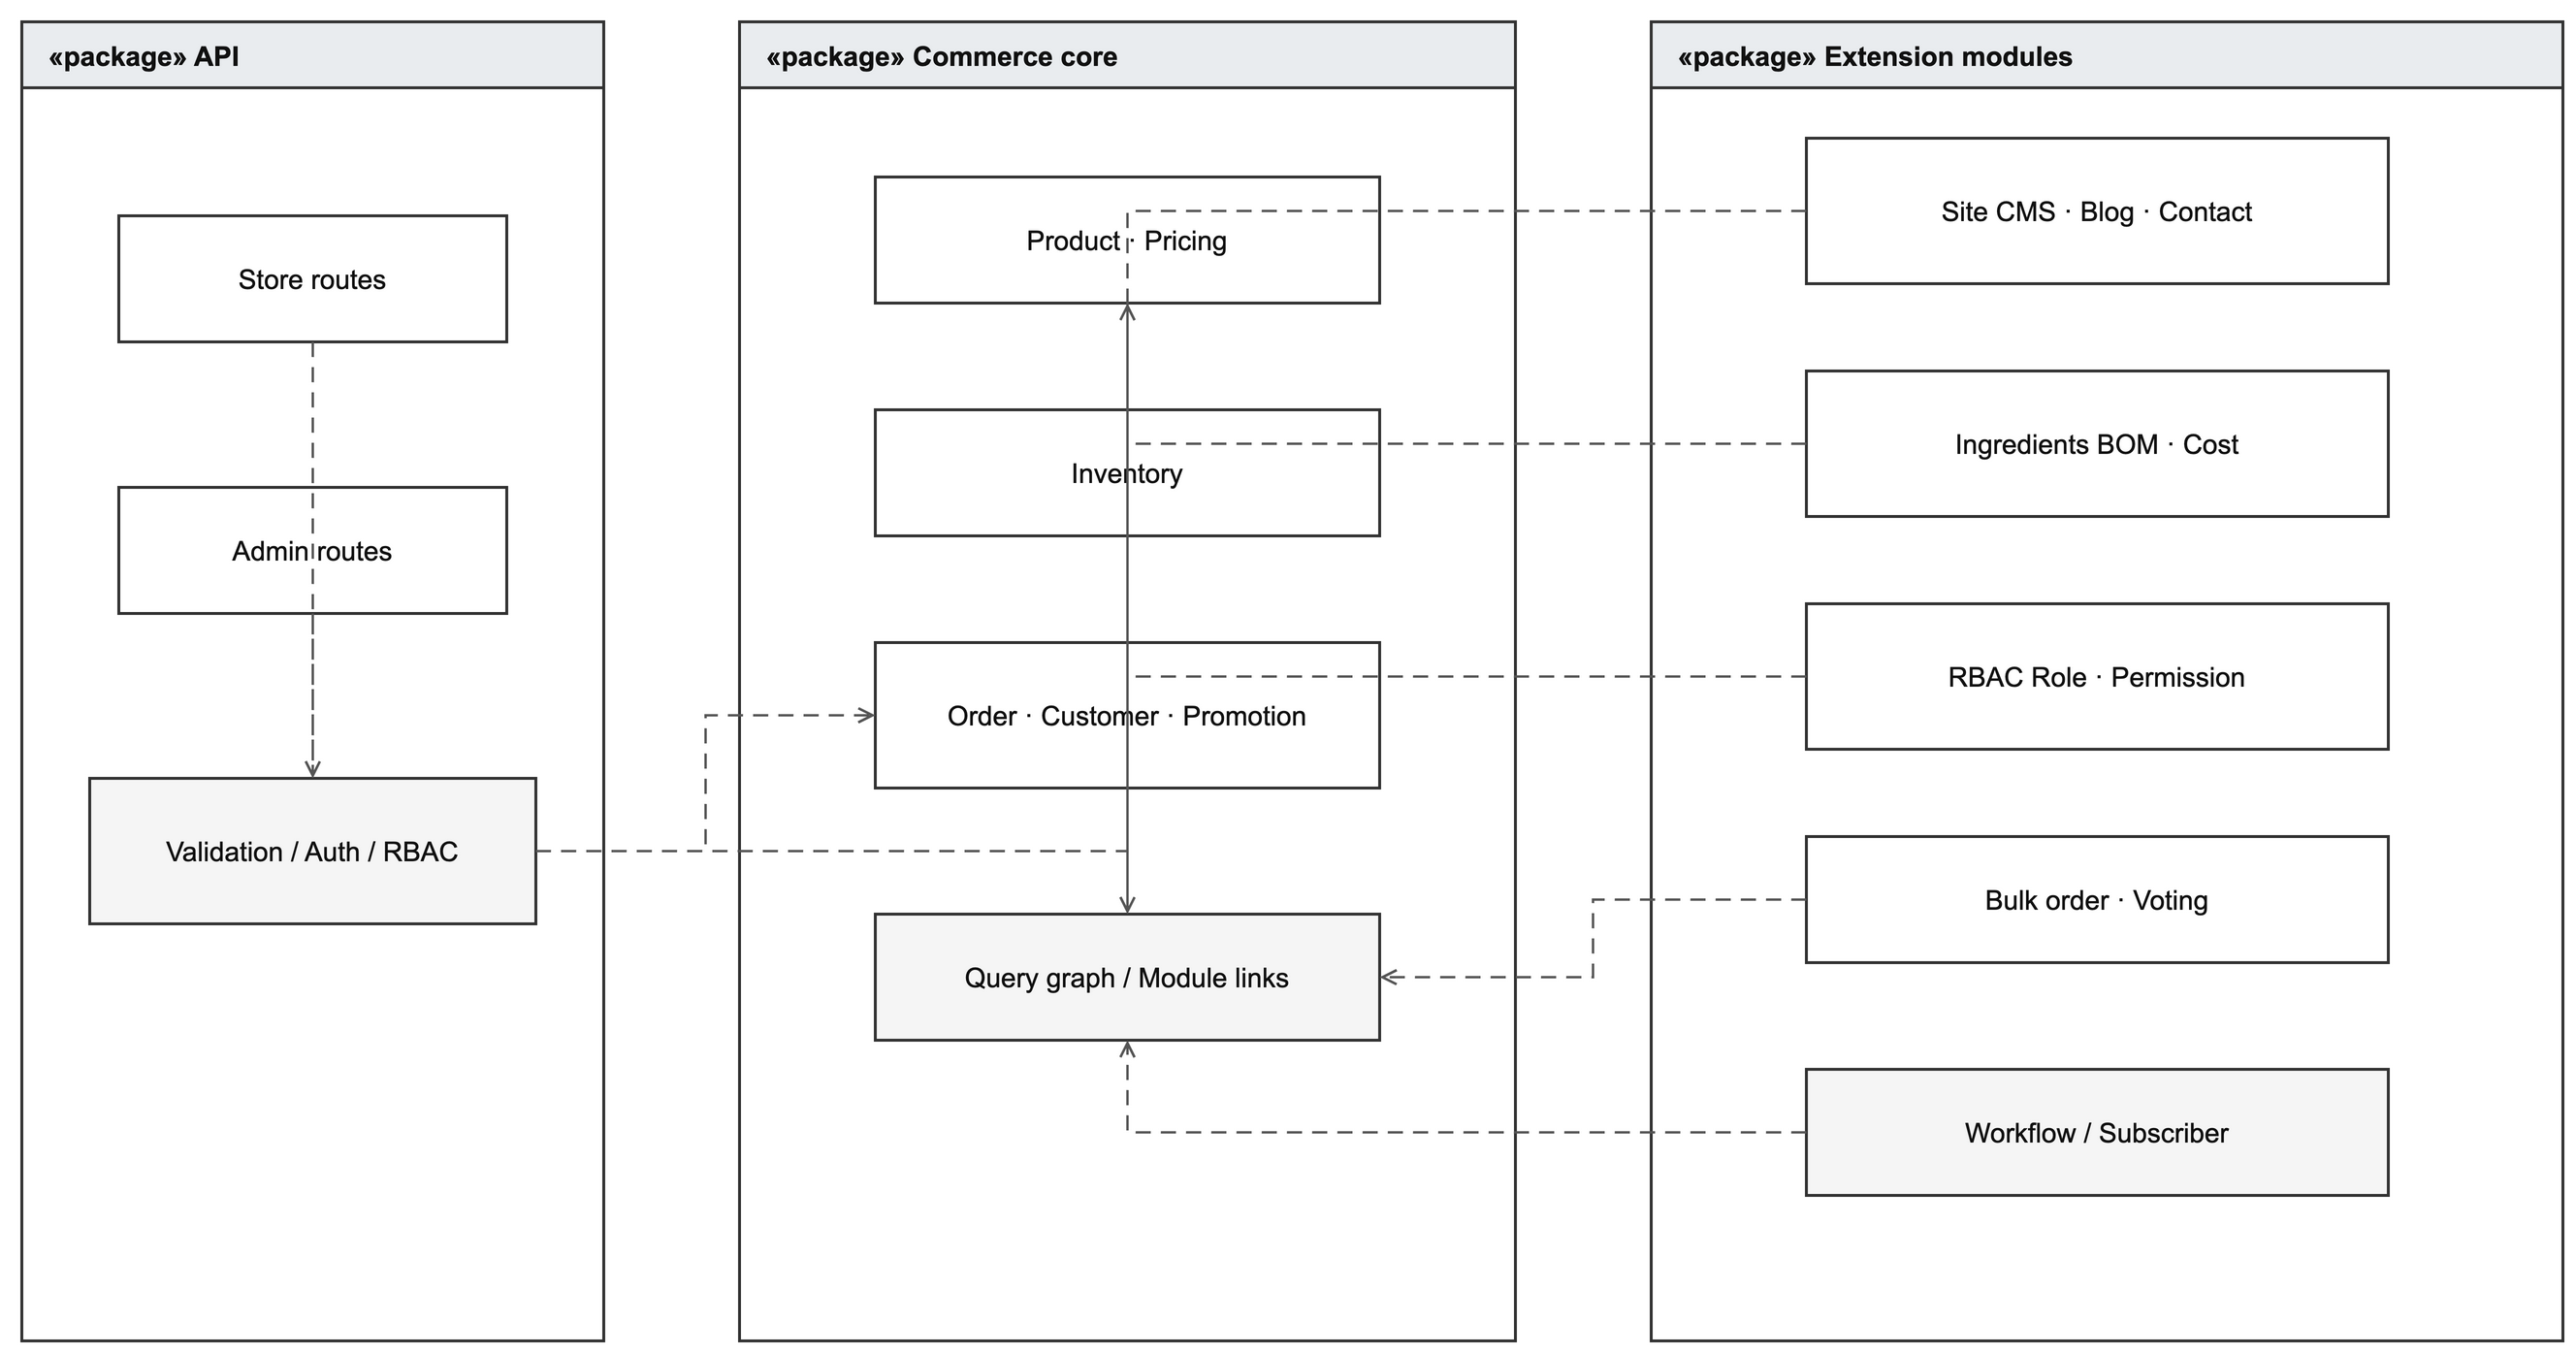
\includegraphics[width=\textwidth,height=0.72\textheight,keepaspectratio]{images/modules.drawio.png}
  \caption{Cấu trúc mô-đun nghiệp vụ và điểm tích hợp}
  \label{fig:module-structure}
\end{figure}

\subsection{API, workflow và subscriber}

API được chia theo hai namespace: \texttt{/store} dành cho khách hàng và \texttt{/admin} dành cho vận hành. Middleware chung thực hiện xác thực, RBAC, validation và chuẩn hóa response. Workflow đã được sử dụng cho luồng tạo contact message. Các thay đổi sản phẩm và đơn hàng được xử lý tiếp bằng subscriber:

\begin{itemize}[leftmargin=2em, itemsep=3pt]
  \item Sản phẩm tạo/cập nhật/xóa sẽ đồng bộ tài liệu tương ứng trong Meilisearch và vô hiệu cache.
  \item Danh mục thay đổi sẽ xóa cache danh mục và cache tìm kiếm.
  \item Đơn được tạo sẽ phát sự kiện \texttt{order.placed}; subscriber trừ tồn nguyên liệu và chuẩn bị email xác nhận.
\end{itemize}

\section{Luồng Checkout}

\subsection{Biểu đồ hoạt động}

Biểu đồ hoạt động trong Hình~\ref{fig:checkout-activity} tách trách nhiệm thành bốn swimlane. Frontend chỉ kiểm tra dữ liệu ở mức giao diện; Checkout API xác minh lại dữ liệu tin cậy; dịch vụ nghiệp vụ chịu trách nhiệm tồn kho, phí giao hàng và khuyến mãi. Hai nút quyết định thể hiện rõ đường thành công và đường quay lại sửa dữ liệu.

\begin{figure}[H]
  \centering
  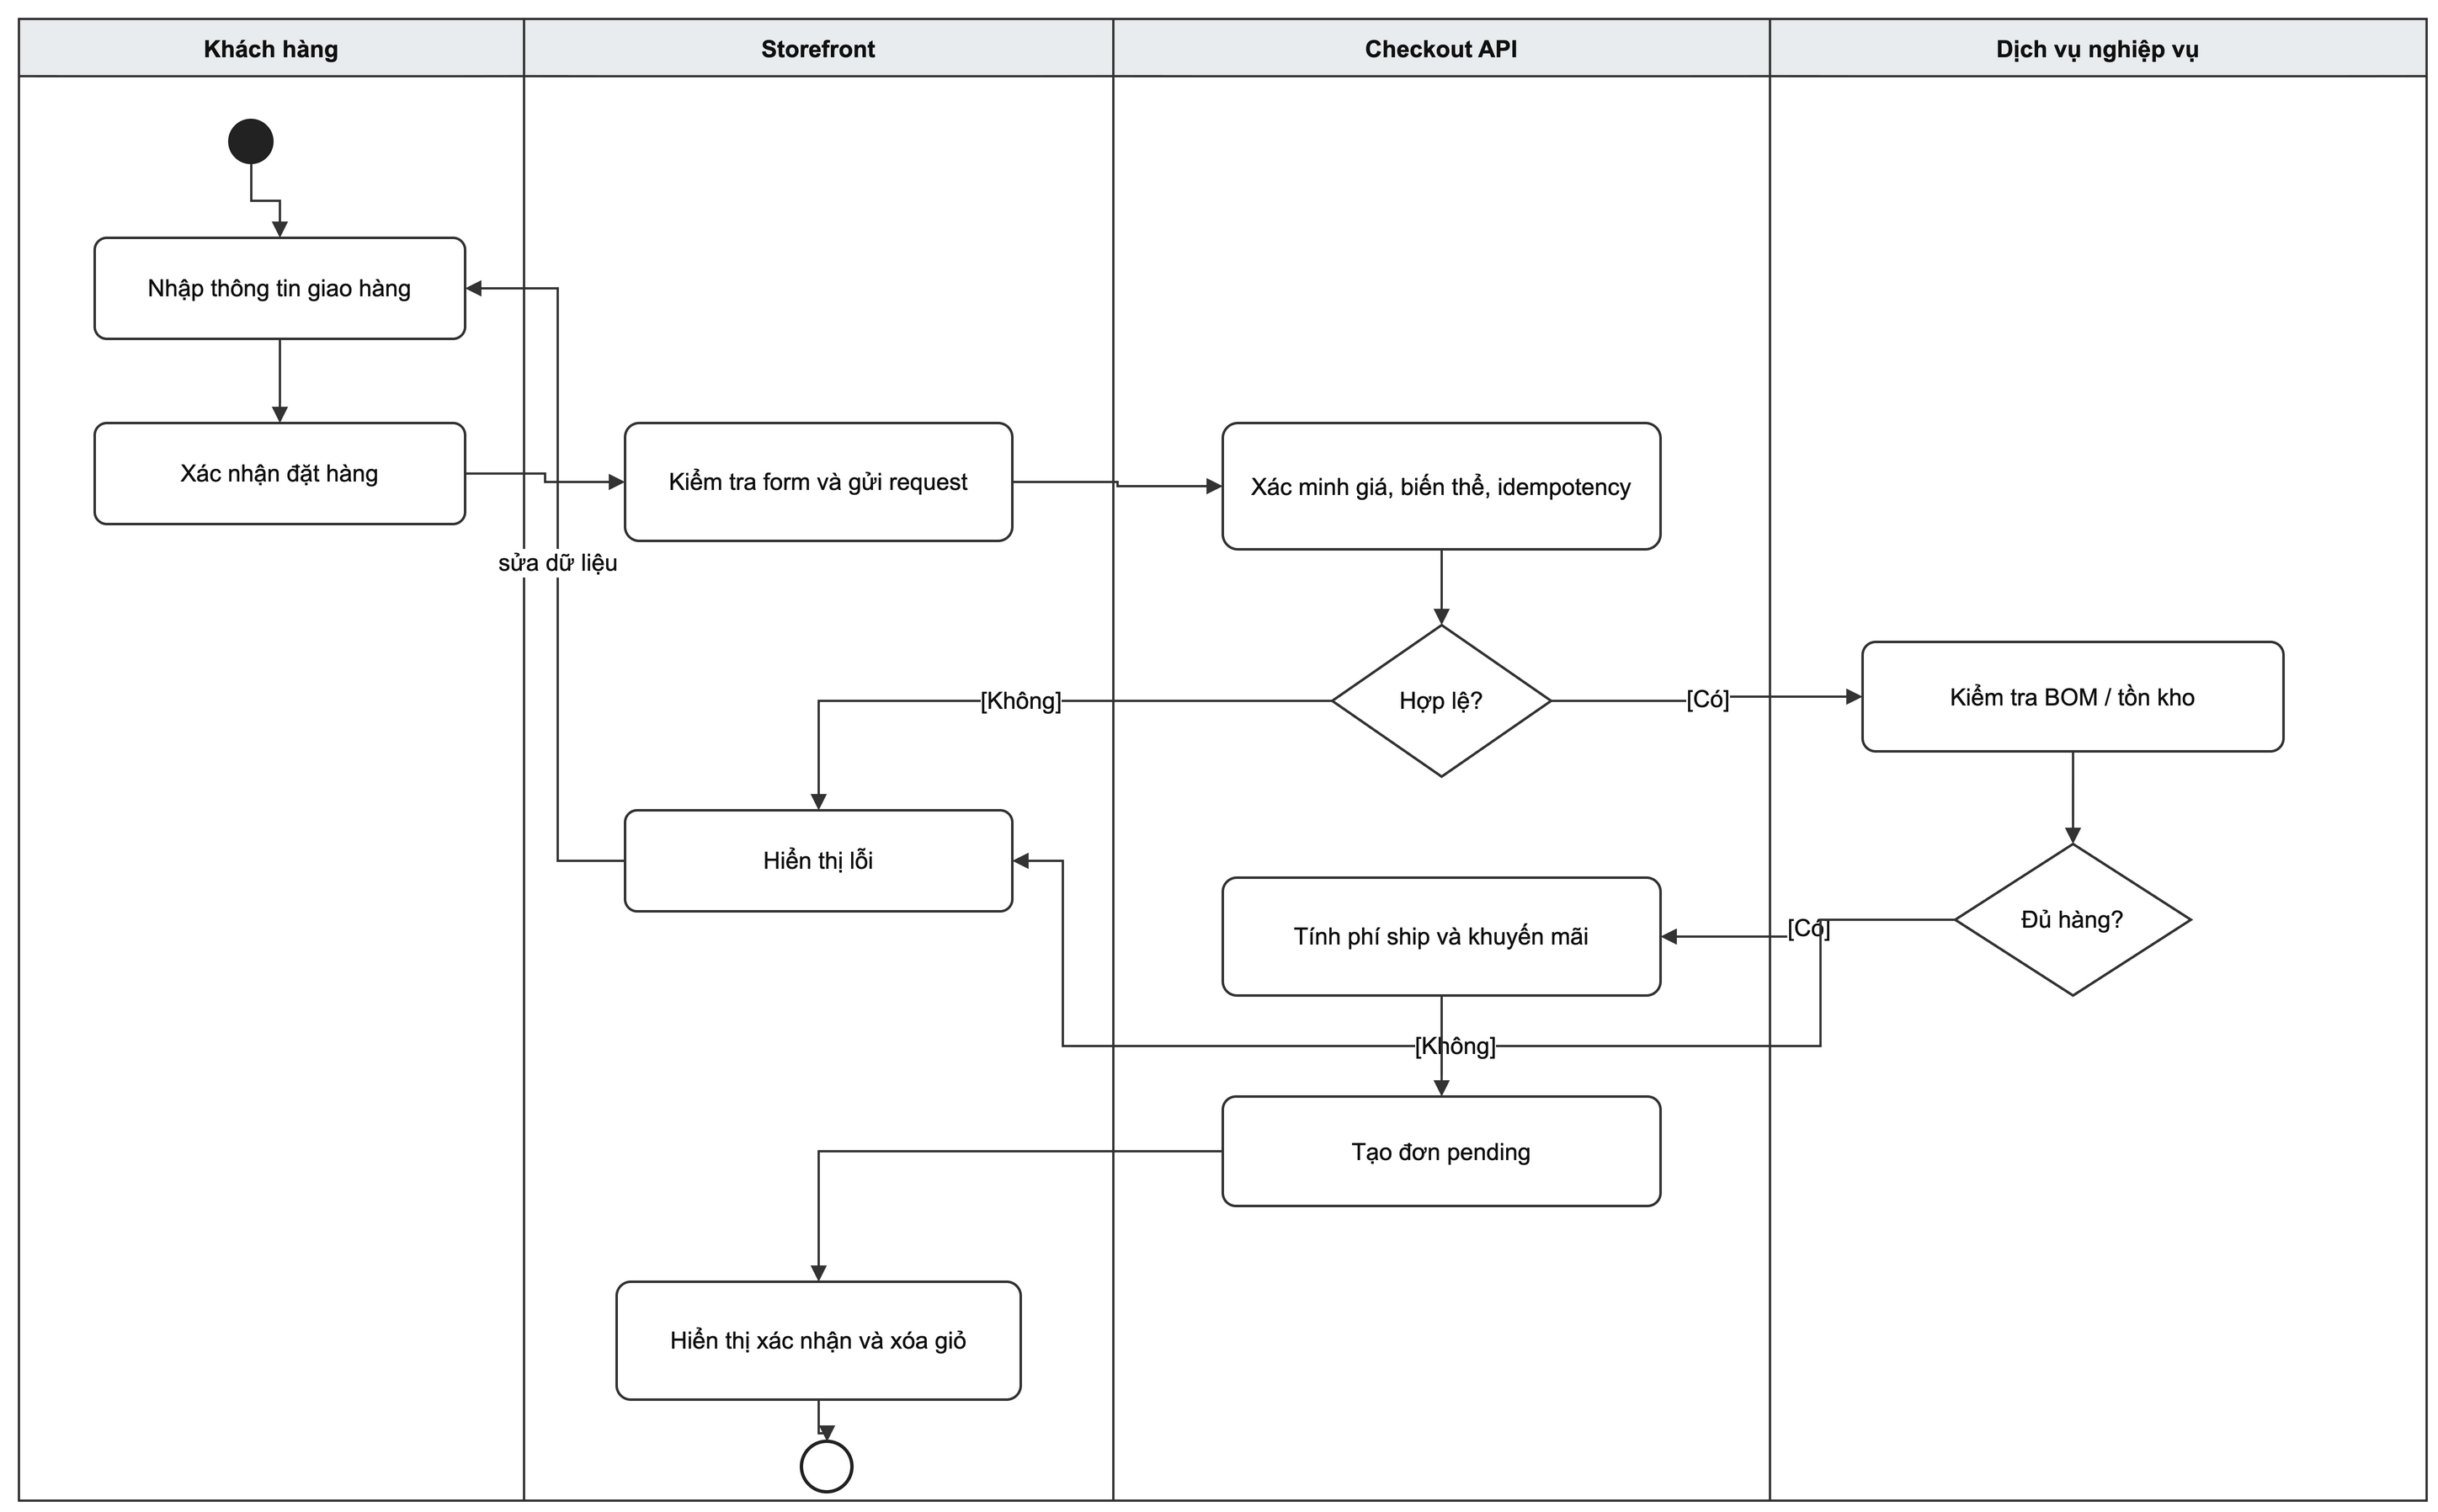
\includegraphics[width=\textwidth,height=0.76\textheight,keepaspectratio]{images/activity-checkout.drawio.png}
  \caption{Biểu đồ hoạt động của quy trình checkout}
  \label{fig:checkout-activity}
\end{figure}

\subsection{Biểu đồ trình tự}

\begin{figure}[H]
  \centering
  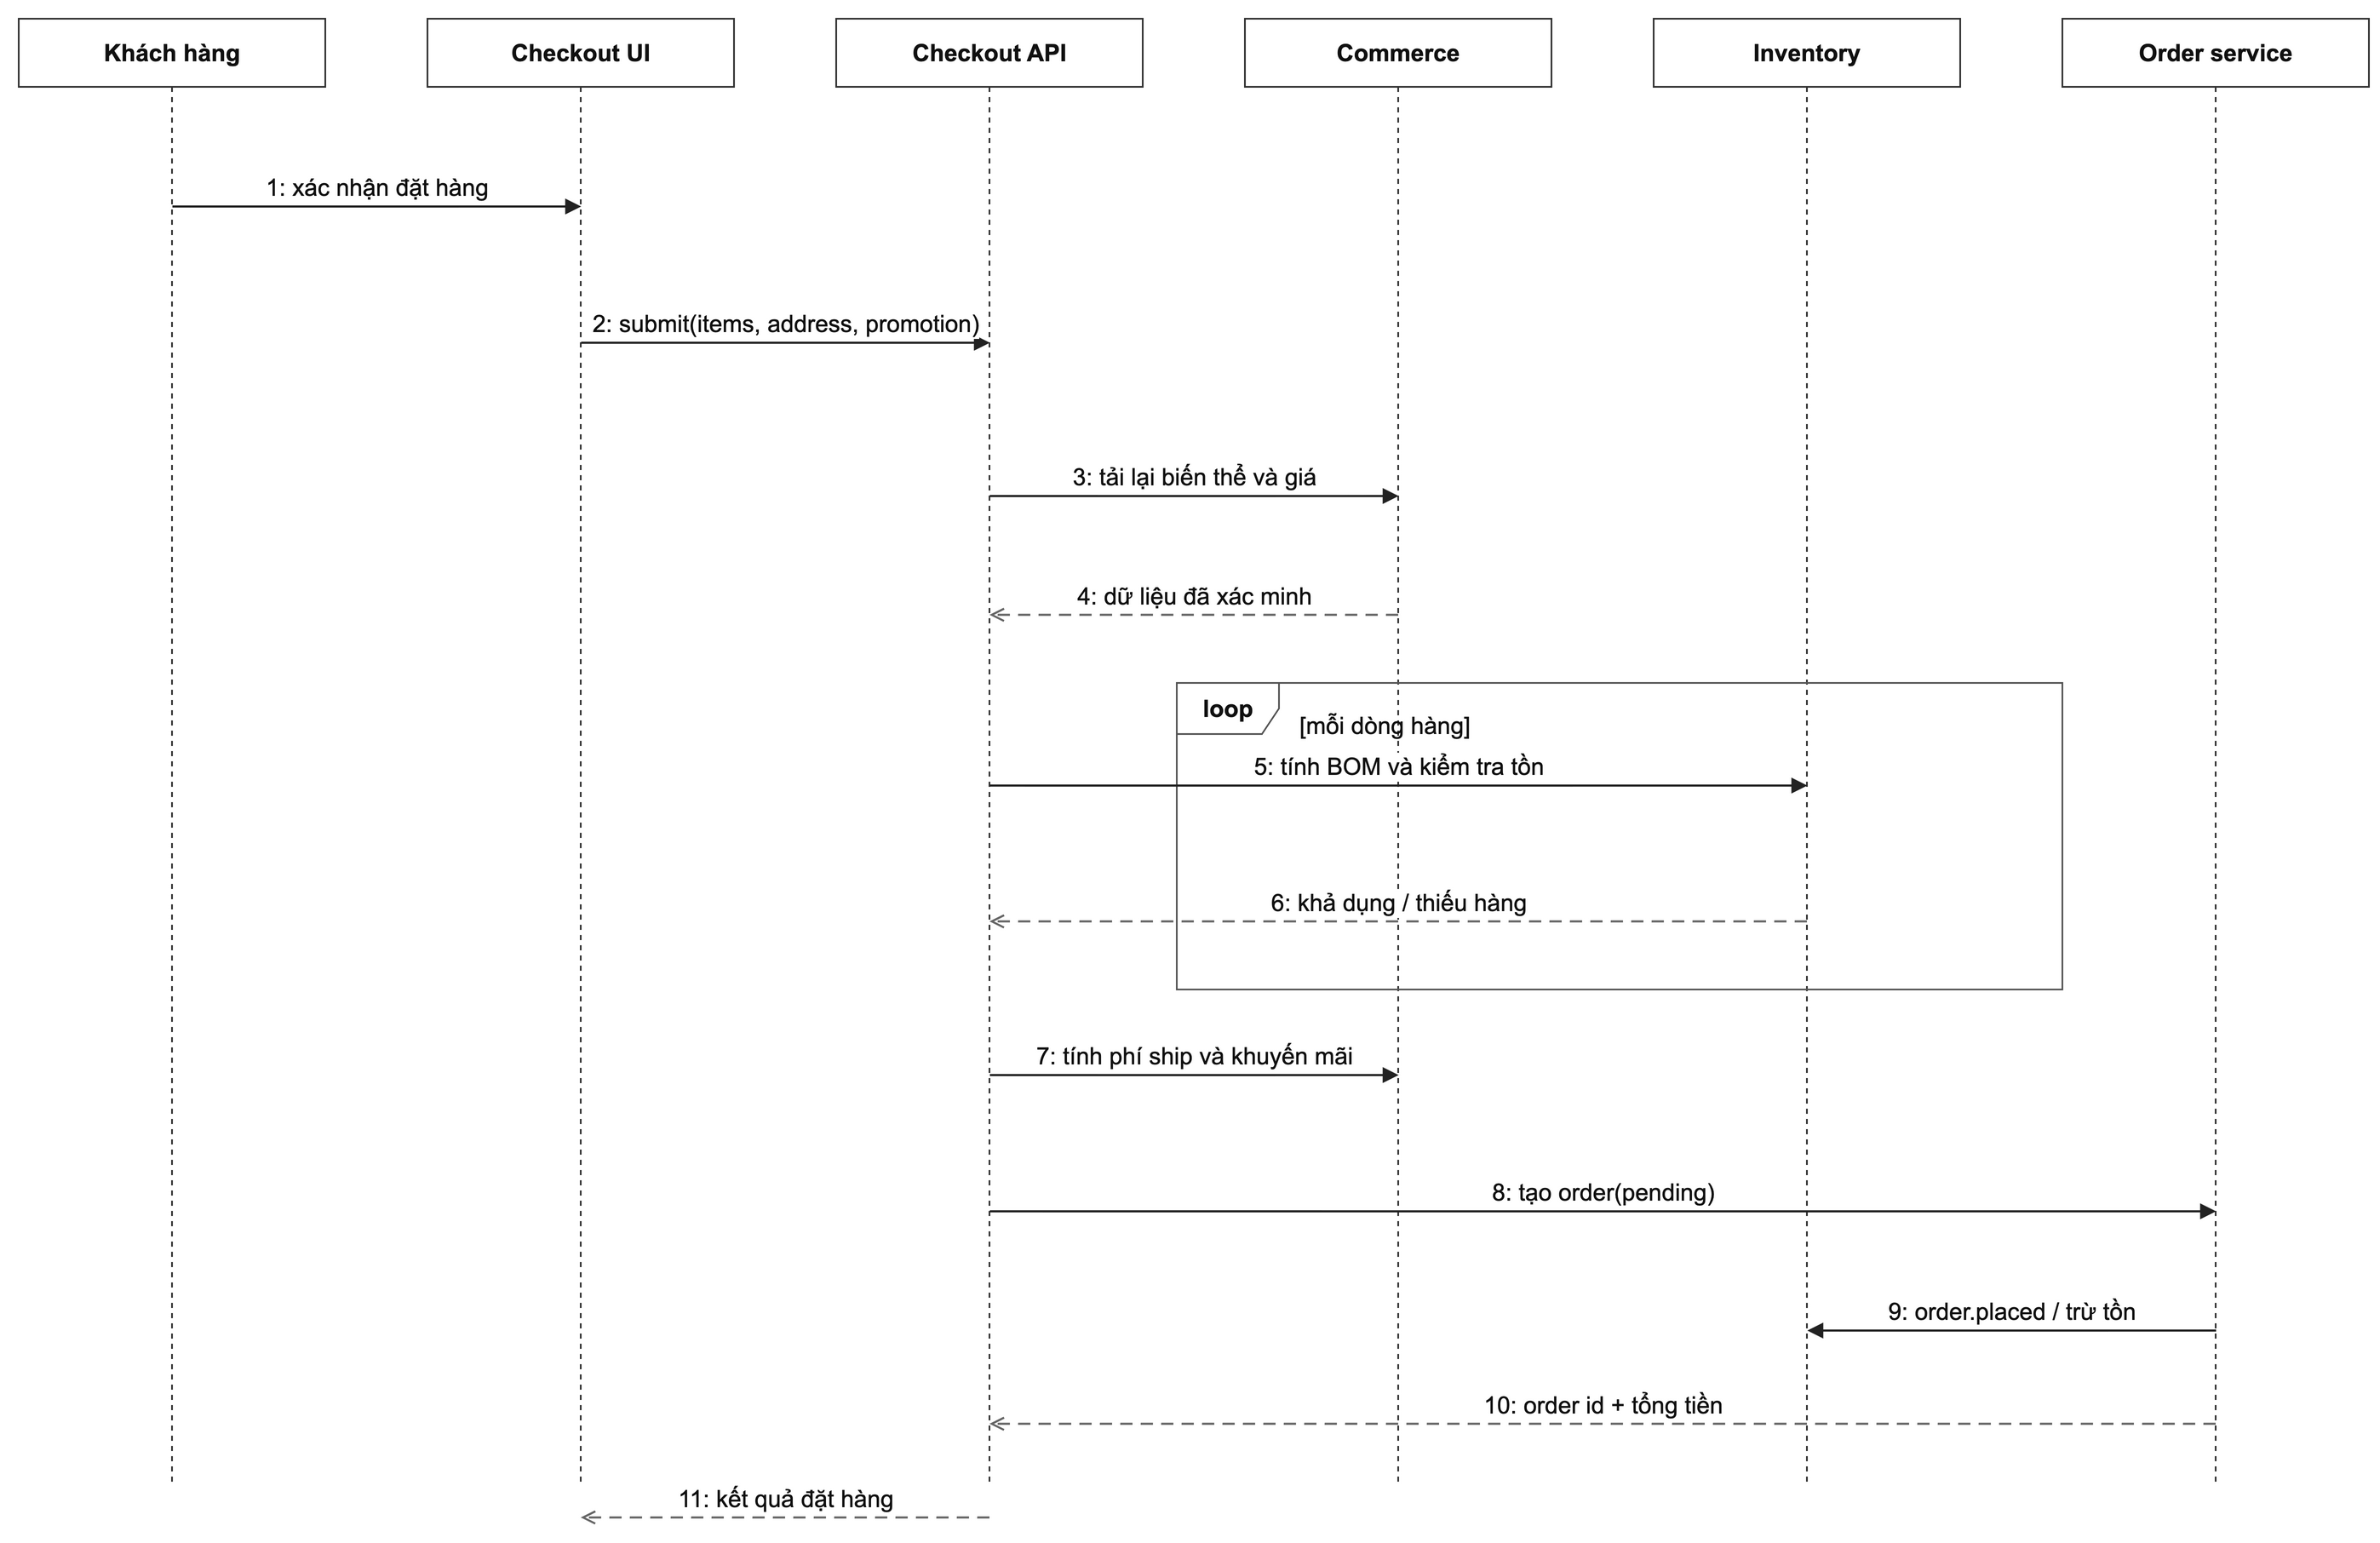
\includegraphics[width=\textwidth,height=0.76\textheight,keepaspectratio]{images/checkout-sequence.drawio.png}
  \caption{Biểu đồ trình tự của luồng xử lý đặt hàng}
  \label{fig:checkout-flow}
\end{figure}

Điểm quan trọng của thiết kế là backend không chấp nhận giá do trình duyệt gửi. Tuy nhiên, route checkout hiện tạo đơn trực tiếp qua service và tự phát sự kiện, tức chưa sử dụng đầy đủ workflow có compensation của Medusa. Đây là điểm cần tái cấu trúc để đảm bảo rollback khi một bước sau tạo đơn thất bại.

\section{Mô Hình Lớp Miền}

Hình~\ref{fig:domain-class} giữ lại các lớp có ảnh hưởng trực tiếp đến catalog, công thức nguyên liệu, đơn hàng và RBAC. Product sở hữu nhiều ProductVariant; mỗi biến thể có nhiều RecipeItem nối tới Ingredient; Ingredient được ánh xạ tới một InventoryItem để theo dõi lượng tồn. Order sở hữu các dòng OrderLineItem và mỗi dòng tham chiếu đúng một biến thể tại thời điểm mua.

\begin{figure}[H]
  \centering
  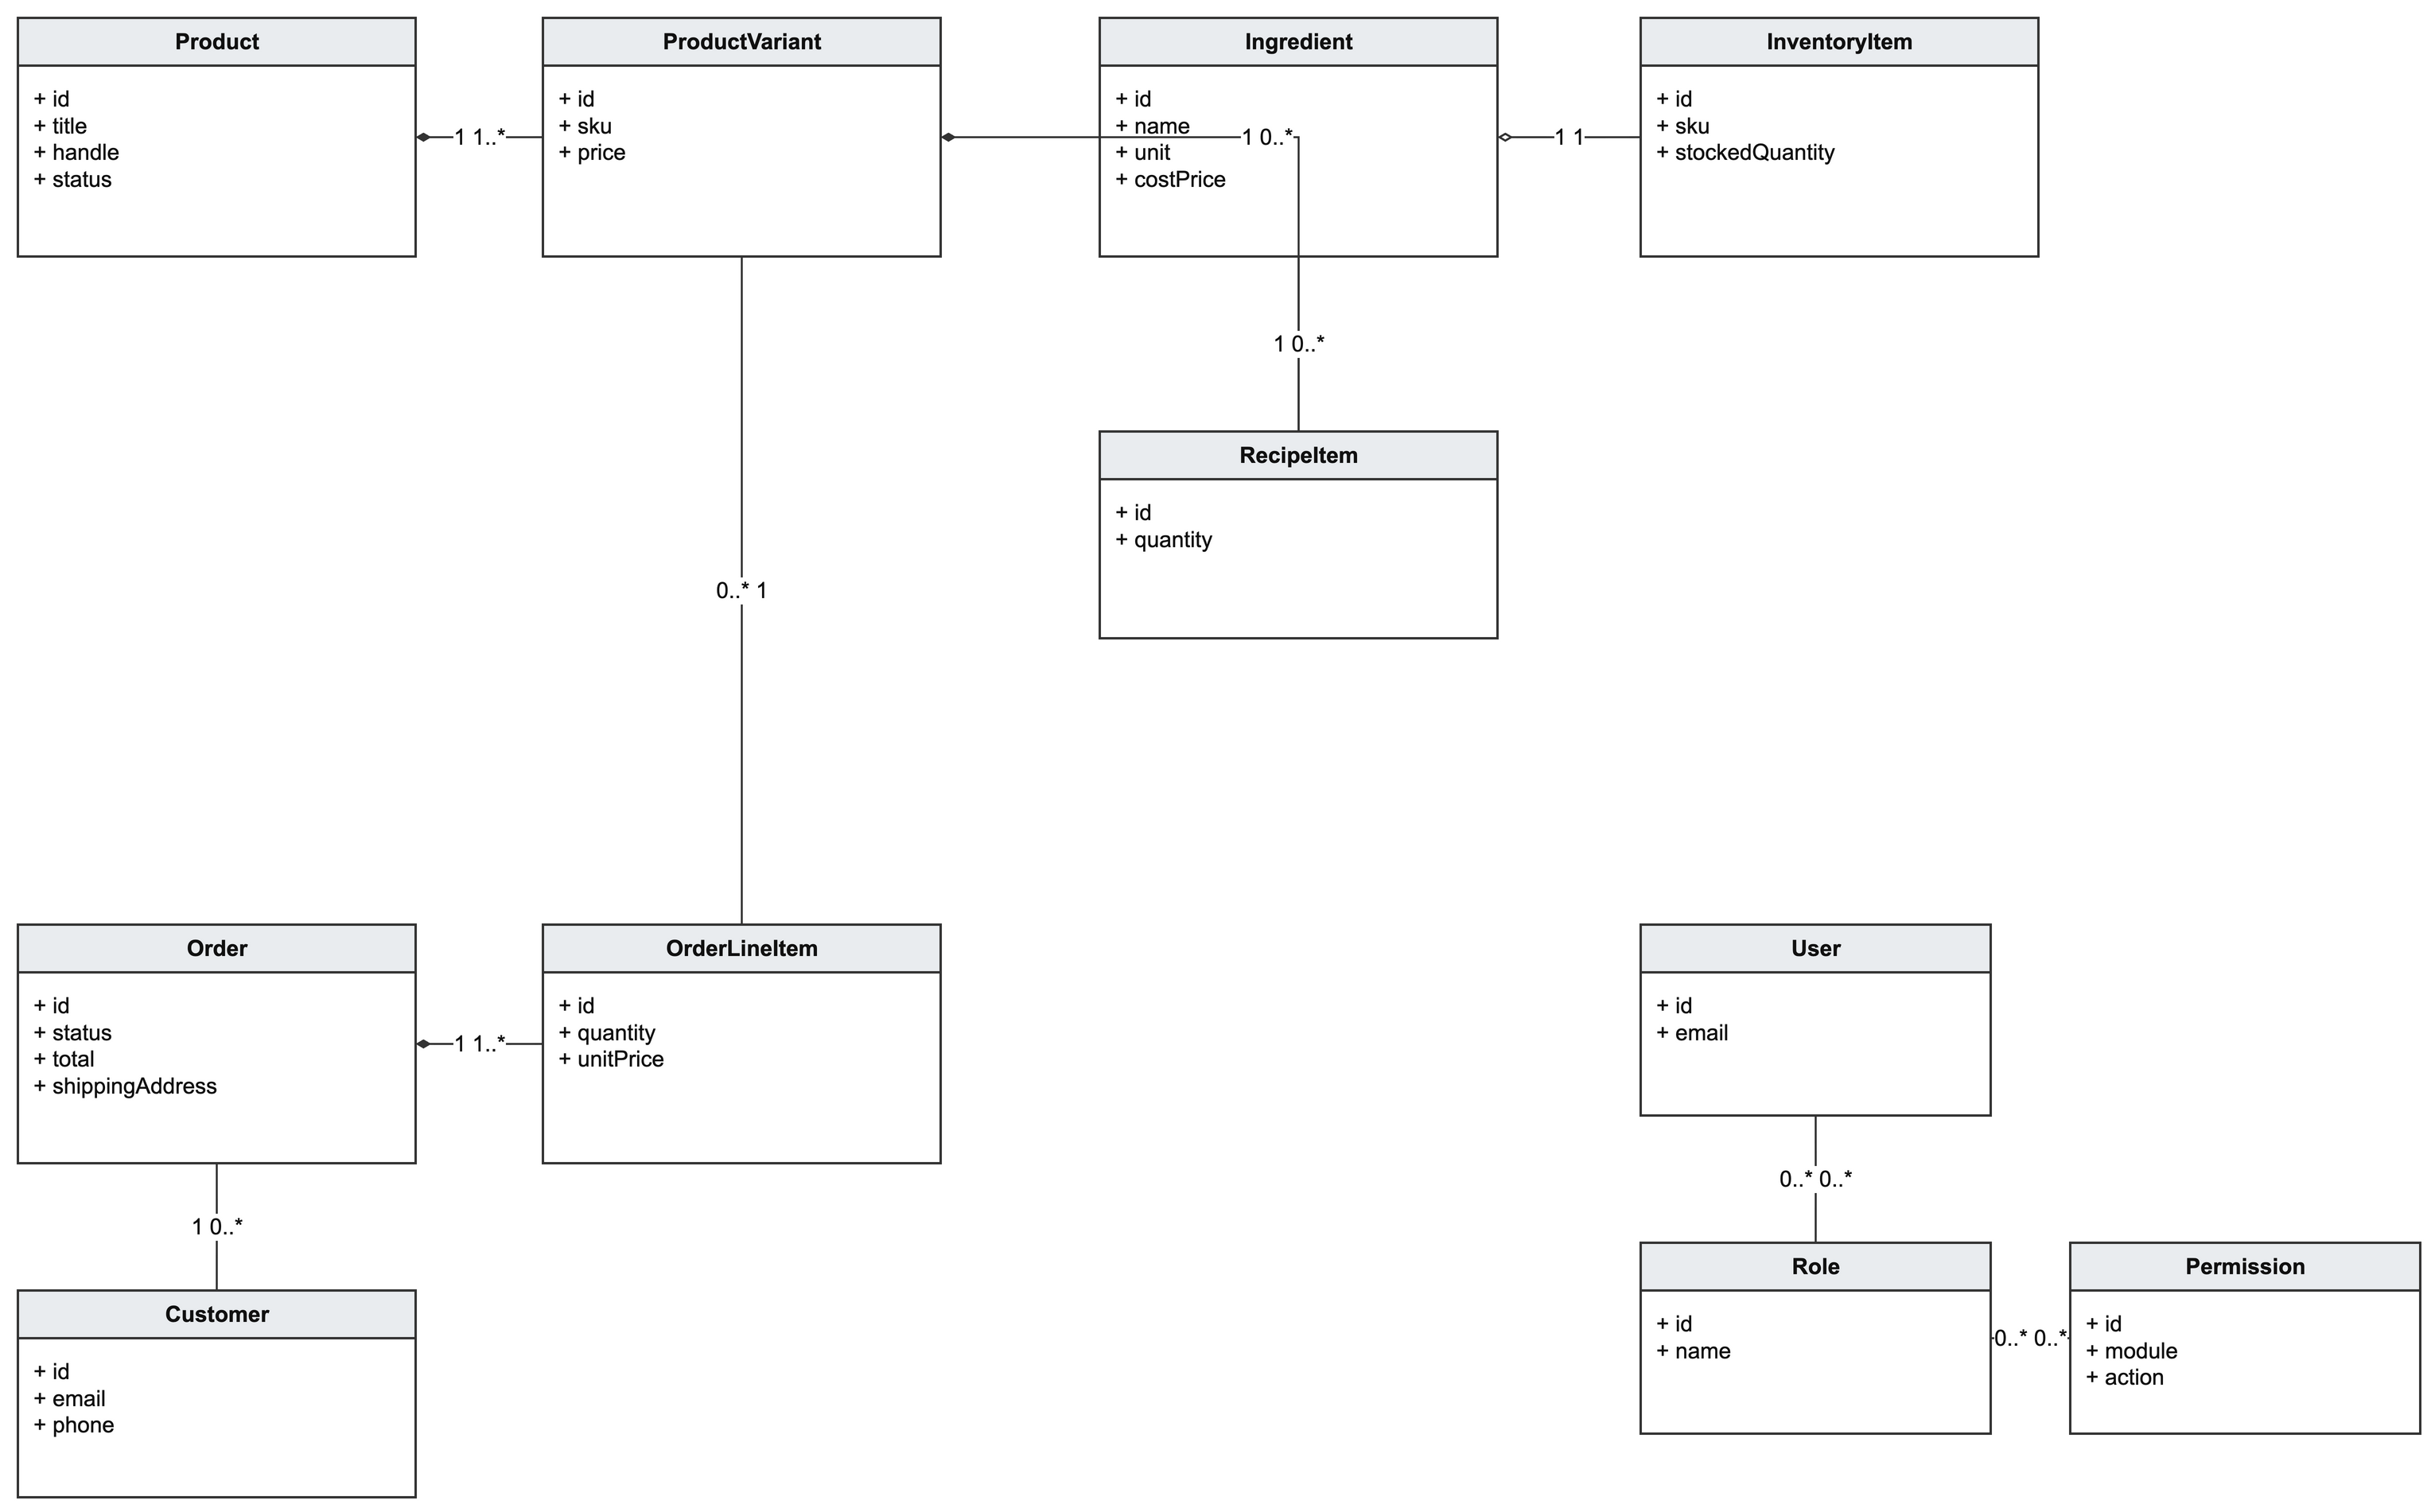
\includegraphics[width=\textwidth,height=0.78\textheight,keepaspectratio]{images/domain-class.drawio.png}
  \caption{Biểu đồ lớp miền nghiệp vụ chính}
  \label{fig:domain-class}
\end{figure}

Các bội số trên quan hệ giúp kiểm tra mô hình trước khi cài đặt. Ví dụ, một Order không nên tồn tại mà không có OrderLineItem; một ProductVariant có thể chưa được cấu hình công thức; Role và Permission có quan hệ nhiều--nhiều. Các lớp trong sơ đồ là mô hình logic, không đồng nghĩa mỗi quan hệ phải được cài bằng khóa ngoại trực tiếp vì Medusa sử dụng module link để bảo toàn ranh giới mô-đun.

\section{Tìm Kiếm và Chatbot}

Tài liệu tìm kiếm chứa tên, mô tả, slug, danh mục, mức giá, giá nhỏ nhất/lớn nhất, ảnh và trạng thái tồn. Subscriber giữ chỉ mục đồng bộ với catalog. Khi tìm kiếm chính không hoạt động, backend xây tài liệu từ Query API và lọc tại ứng dụng.

Chatbot sử dụng mô hình retrieval-augmented generation ở mức đơn giản: truy vấn FAQ và sản phẩm liên quan, tạo system prompt có giới hạn quyền hạn, sau đó gọi Groq. Response được cache 12 giờ theo câu hỏi. Log lưu message đã chuẩn hóa, chế độ phản hồi, trạng thái resolved và số gợi ý; nhờ đó quản trị viên có thể bổ sung FAQ cho câu hỏi chưa được giải quyết.

\begin{figure}[H]
  \centering
  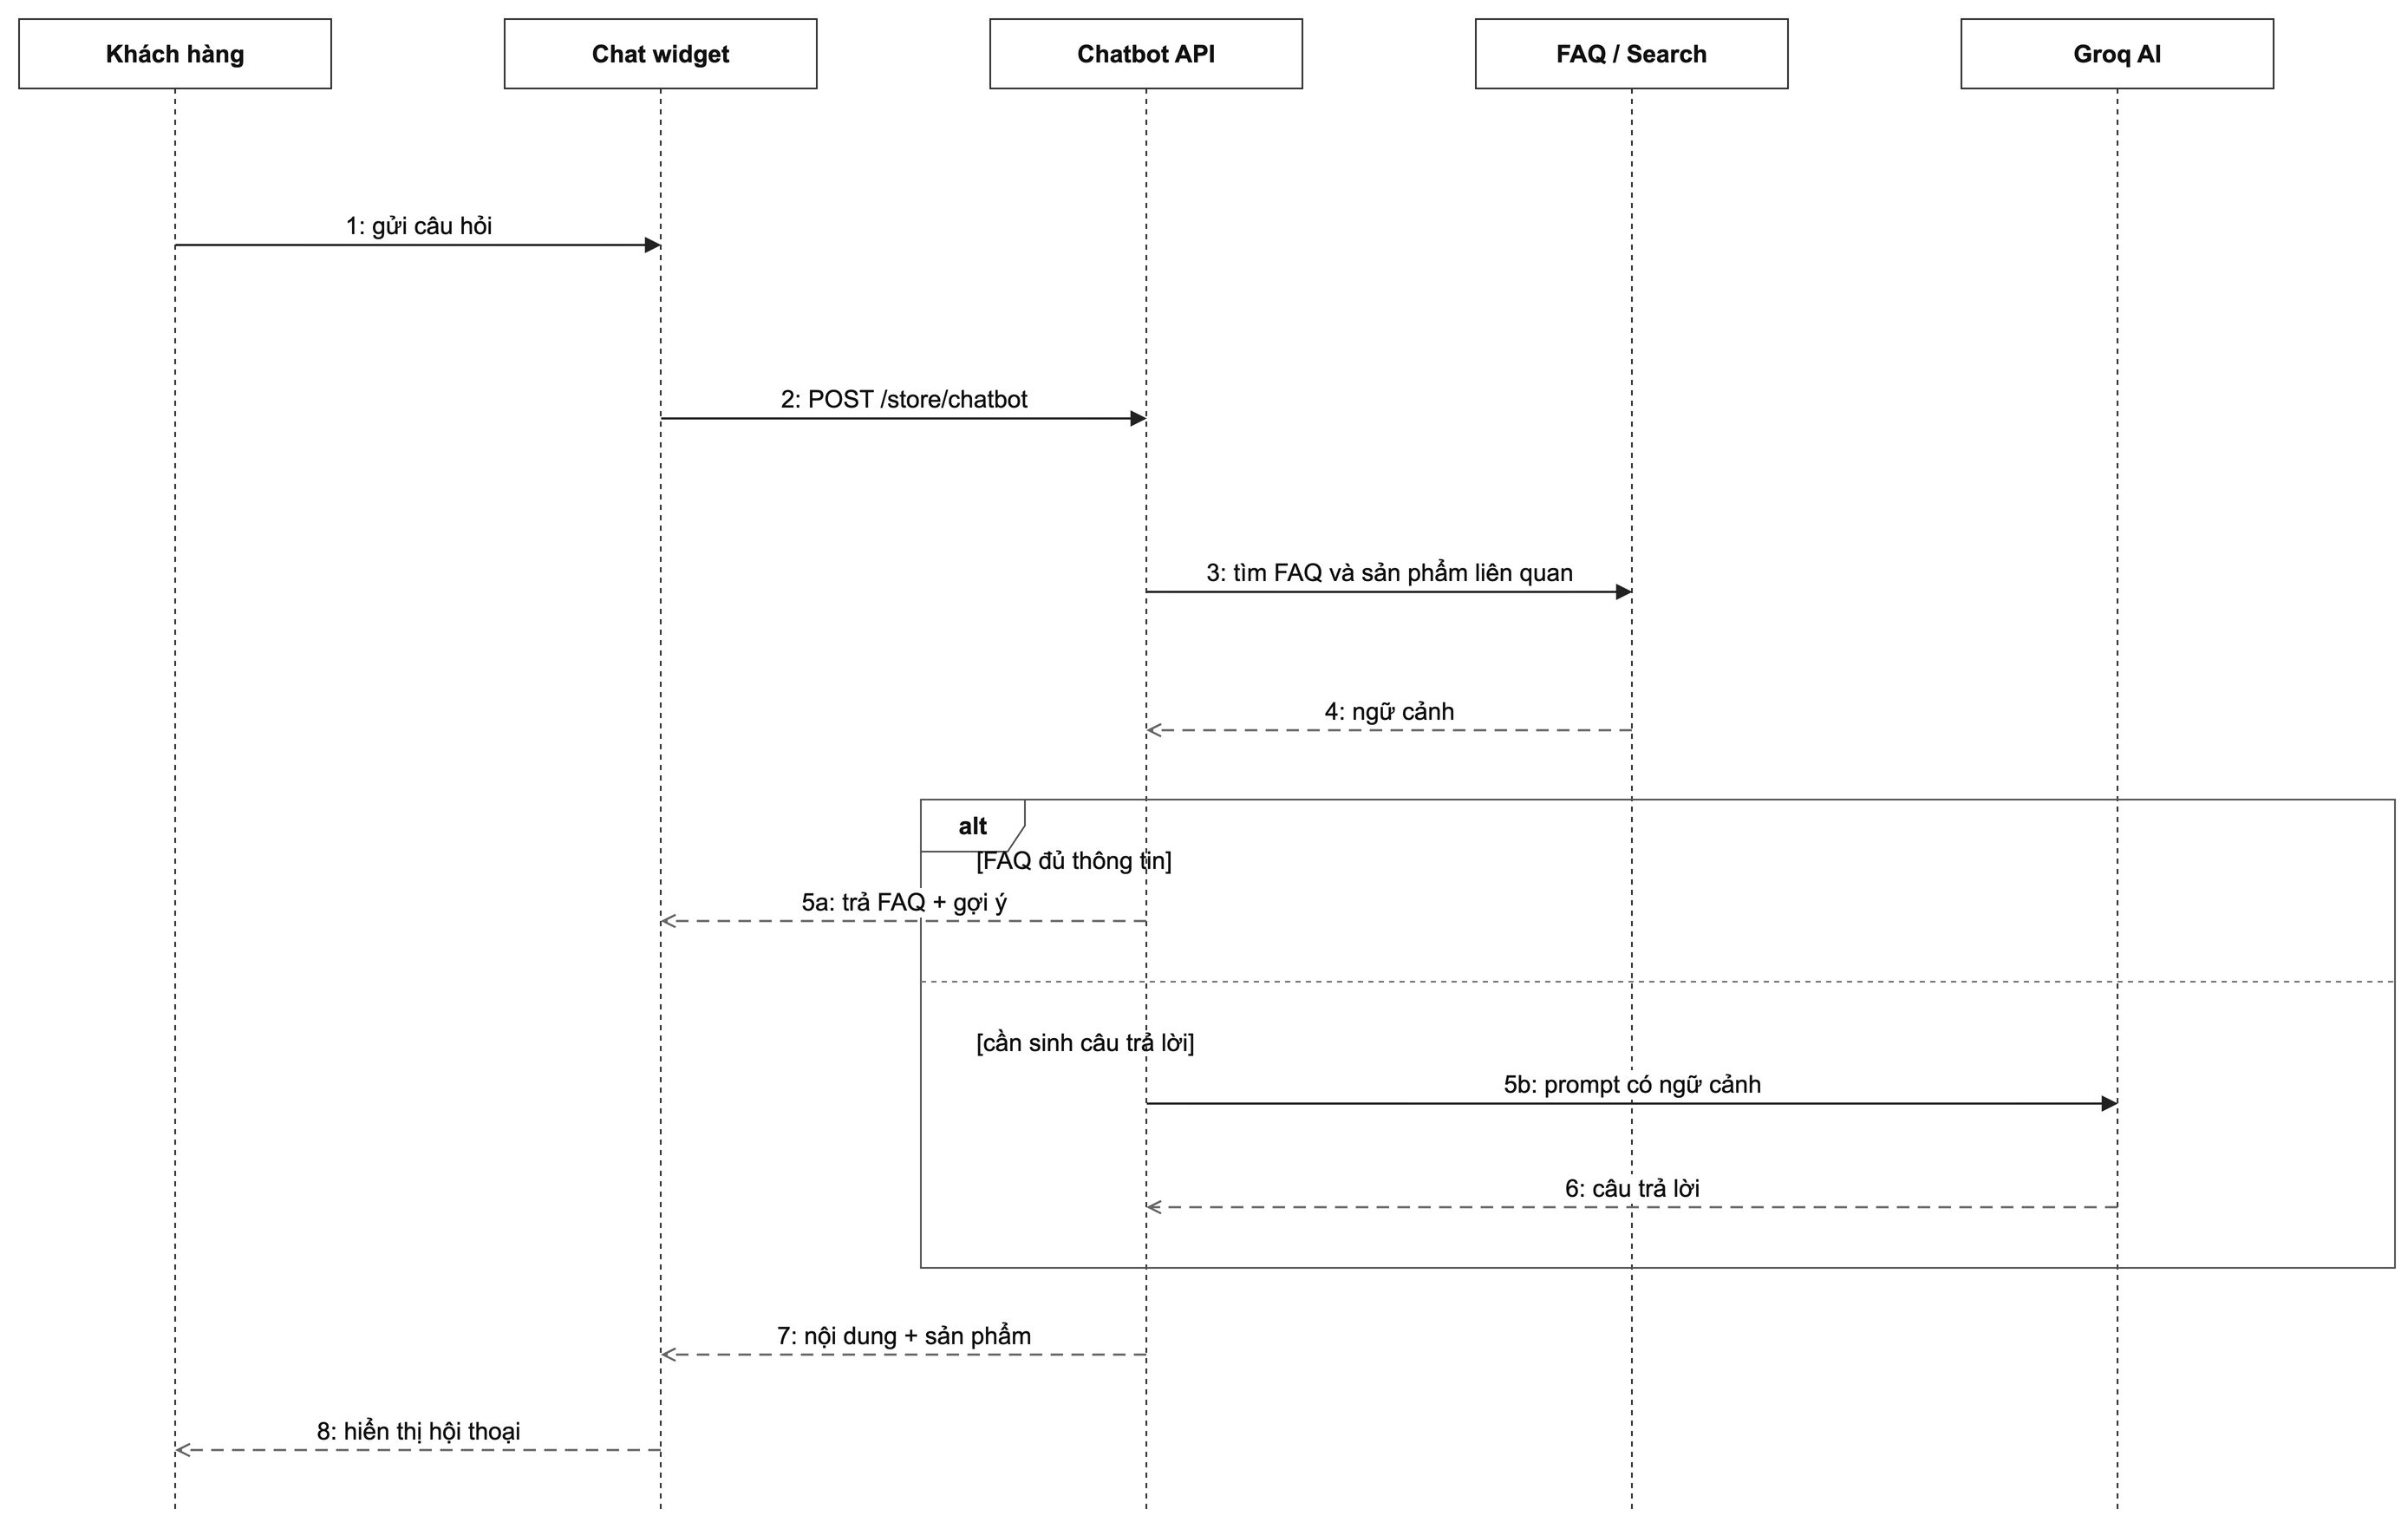
\includegraphics[width=\textwidth,height=0.74\textheight,keepaspectratio]{images/chatbot-sequence.drawio.png}
  \caption{Biểu đồ trình tự của chatbot tư vấn sản phẩm}
  \label{fig:chatbot-sequence}
\end{figure}

\section{Bảo Mật}

\begin{itemize}[leftmargin=2em, itemsep=4pt]
  \item JWT tách riêng cho khách hàng và người dùng quản trị; token hết hạn bị xóa khỏi localStorage.
  \item API admin sử dụng middleware xác thực và RBAC; quyền được kiểm tra lại ở backend, không chỉ dựa vào việc ẩn menu.
  \item Checkout khách được cho phép nhưng không tự liên kết với customer có cùng email, tránh chiếm quyền lịch sử đơn.
  \item Chatbot có rate limit, phạm vi dữ liệu hạn chế và quy tắc chống prompt injection cơ bản.
  \item CORS, JWT secret, cookie secret và khóa dịch vụ được cấu hình bằng biến môi trường.
\end{itemize}

\section{Vòng Đời Đơn Hàng}

Trạng thái đơn được mô hình hóa riêng để tránh cập nhật tùy ý từ giao diện quản trị. Luồng chuẩn đi từ \texttt{pending} tới \texttt{confirmed}, \texttt{processing}, \texttt{shipping} và \texttt{completed}. Hủy đơn chỉ hợp lệ trước khi giao; lỗi giao vận hoặc xử lý có thể chuyển sang \texttt{failed} và được retry có kiểm soát.

\begin{figure}[H]
  \centering
  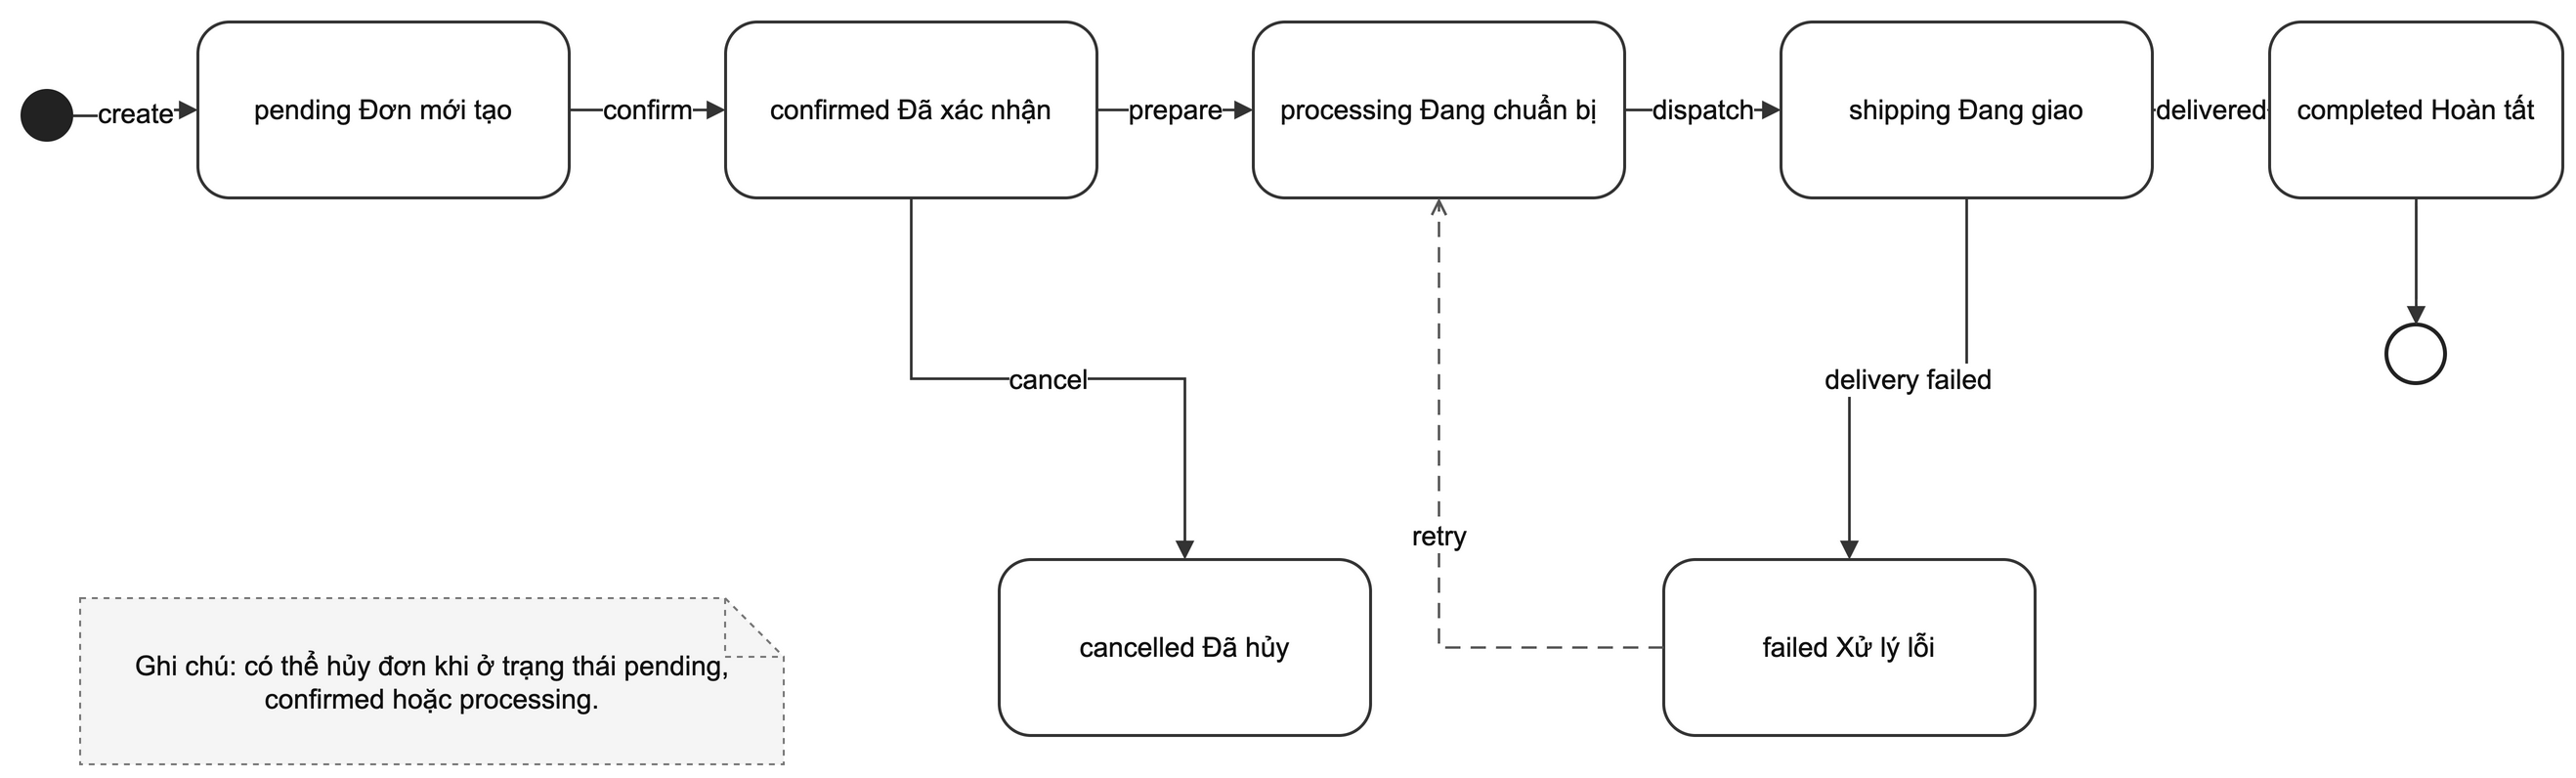
\includegraphics[width=\textwidth,height=0.55\textheight,keepaspectratio]{images/order-state.drawio.png}
  \caption{Biểu đồ trạng thái đơn hàng}
  \label{fig:order-state}
\end{figure}

Mỗi chuyển tiếp nên được thực hiện qua một command hoặc workflow có kiểm tra trạng thái nguồn, quyền người thao tác và tác dụng phụ tương ứng. Cách này ngăn các chuyển tiếp vô nghĩa như đưa đơn đã hoàn tất quay lại xử lý, đồng thời tạo điểm rõ ràng để phát sự kiện, ghi audit log và gửi thông báo.

\section{Mô Hình Triển Khai}

Trong môi trường phát triển, Docker Compose chạy bốn dịch vụ: PostgreSQL cổng 5432, Redis cổng 6379, Meilisearch cổng 7700 và MinIO (S3 API được ánh xạ ra cổng 9001, console cổng 9002). Backend chạy ở cổng 9000; frontend Vite hiện cấu hình cổng 5173 và proxy các đường dẫn \texttt{/auth}, \texttt{/store}, \texttt{/admin}, \texttt{/media} tới backend.

\begin{figure}[H]
  \centering
  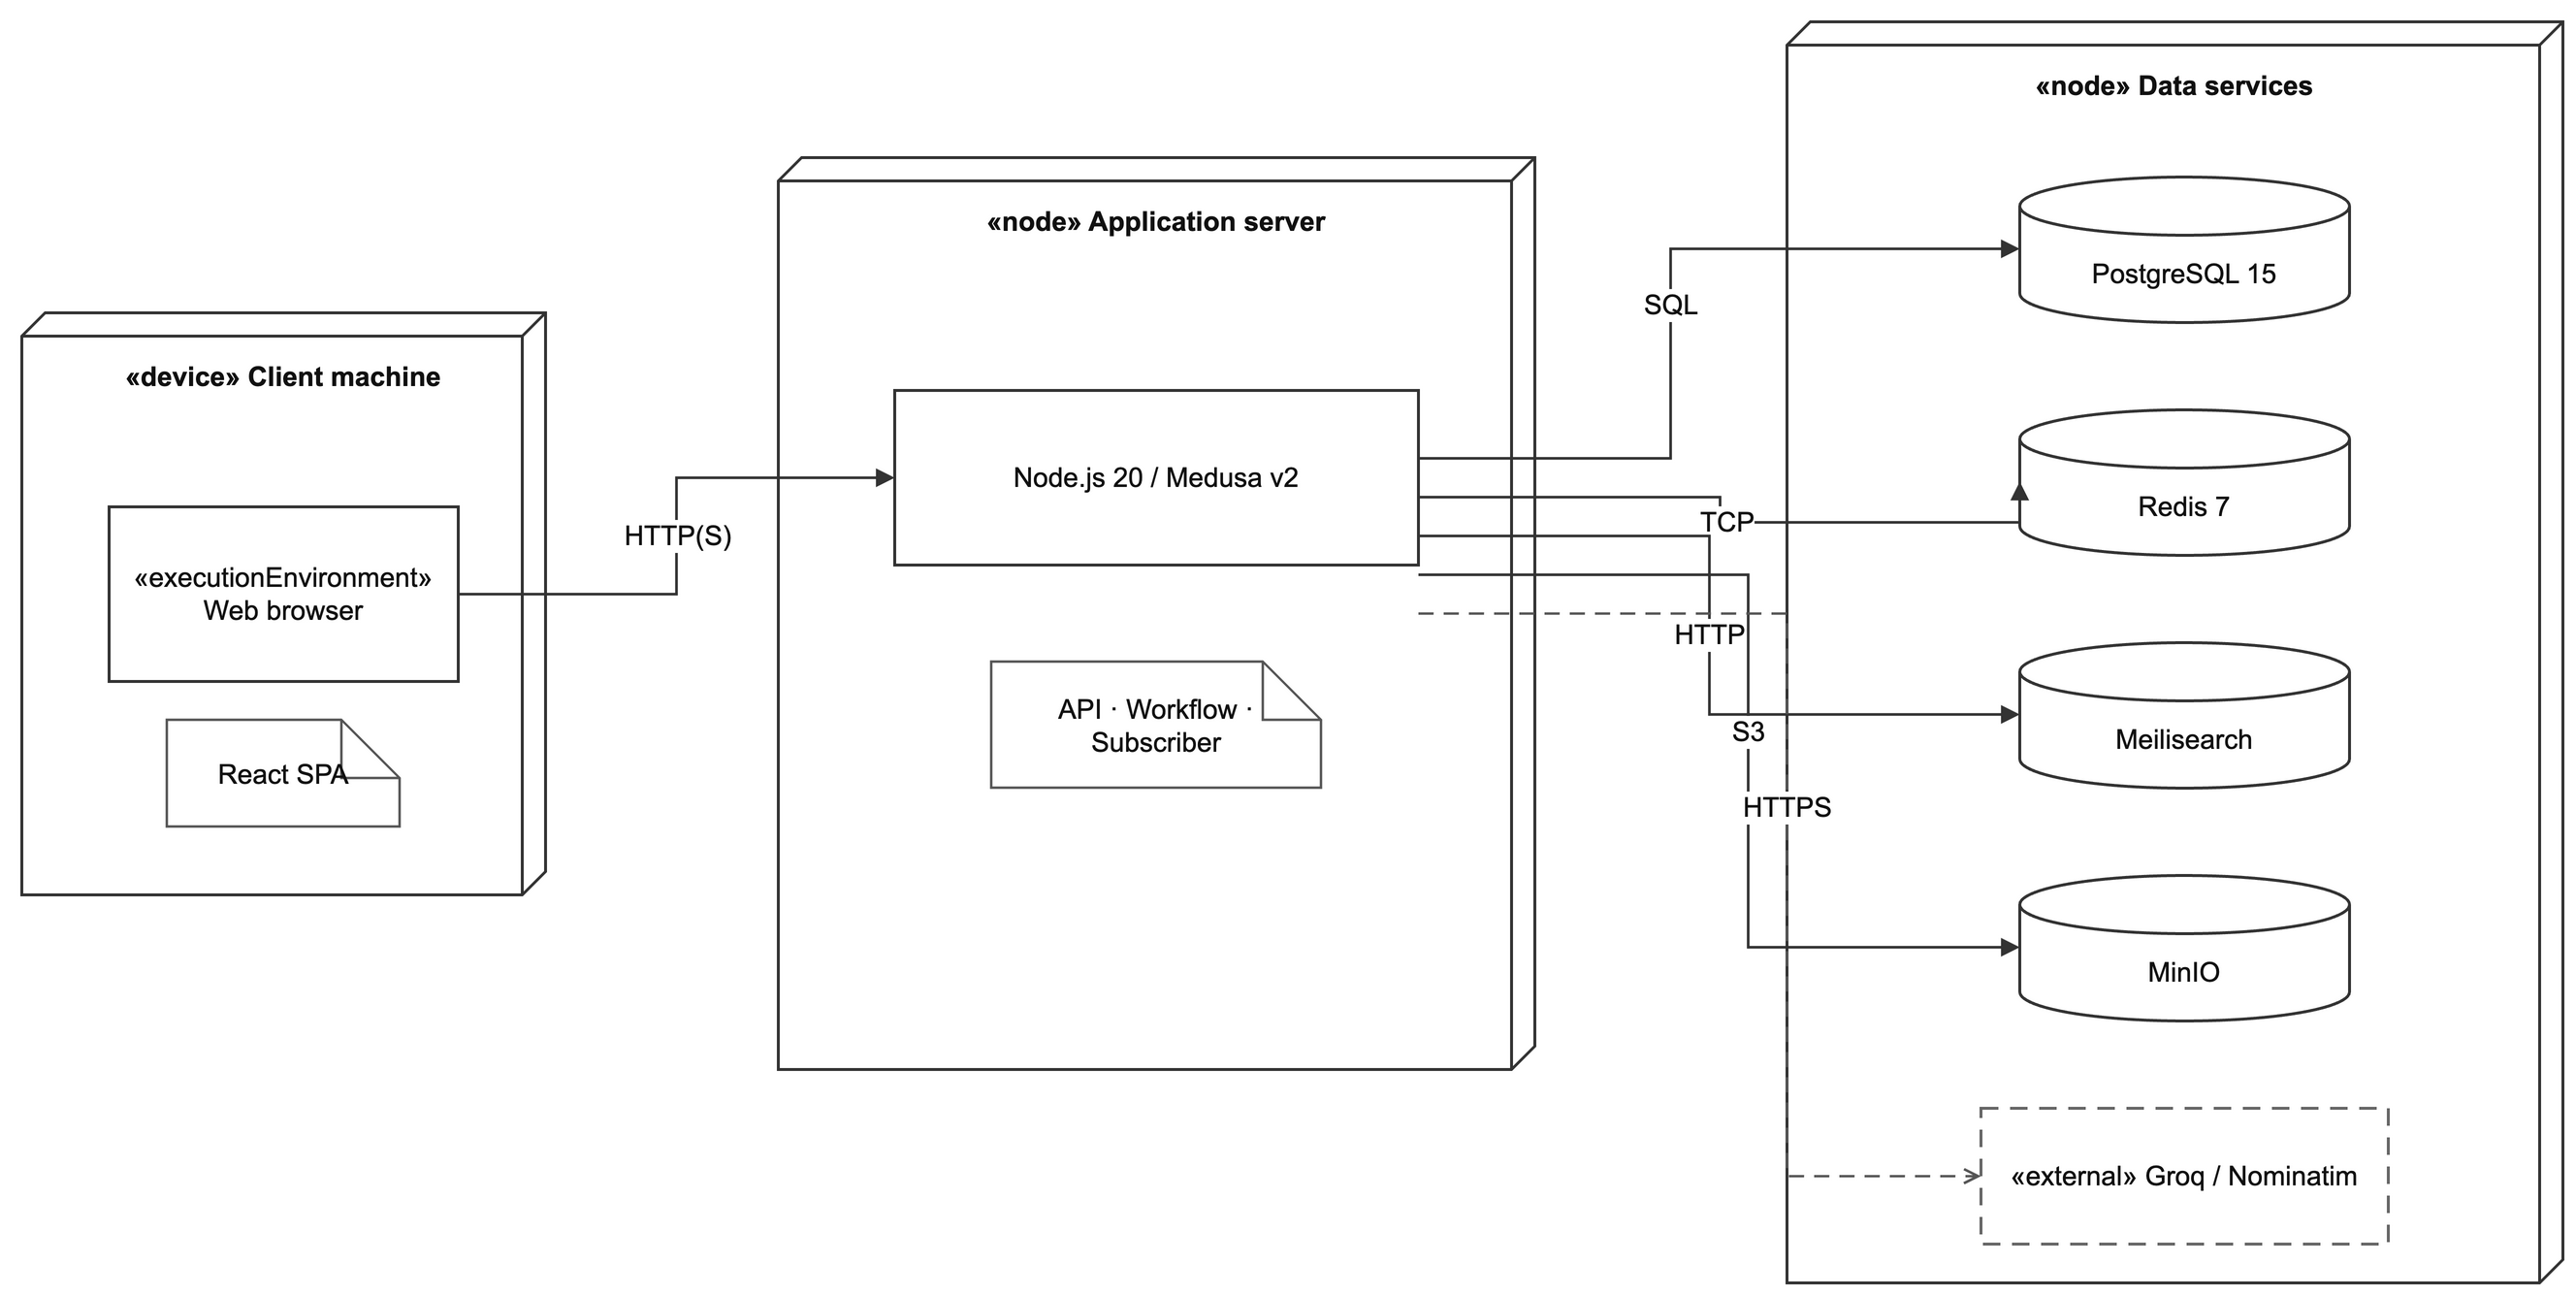
\includegraphics[width=\textwidth,height=0.70\textheight,keepaspectratio]{images/deployment.drawio.png}
  \caption{Mô hình triển khai và các dịch vụ tích hợp}
  \label{fig:deployment}
\end{figure}

Ở production, cần tách secret khỏi mã nguồn, bật HTTPS, giới hạn truy cập Meilisearch/MinIO, cấu hình Redis thật cho cache/event bus và đặt reverse proxy trước hai ứng dụng.
